\section{Introduction}\label{sec:introduction}

Test-time compute scaling, including self-consistency \cite{wang2023selfconsistency}, best-of-$N$ \cite{snell2025scaling, brown2024monkeys}, and extended reasoning \cite{muennighoff2025s1}, has become a reliable strategy for improving reasoning accuracy: sample multiple candidates, estimate quality, select the best.
This approach succeeds when outputs admit equivalence classes or execution-based verification.
For NER, outputs are entity sets with partial overlap, and the boundary conditions for effective scaling remain unknown.
Prior work reports task-level correlations between consistency and accuracy \cite{yao2026consistency} and documents diversity collapse under constrained decoding \cite{yun2025price}, but neither provides instance-level diagnostics that explain \textit{when} scaling helps and \textit{when} it harms.

We study this question across four NER benchmarks and two model families (7--14B fine-tuned, with ablations to 72B), using RE as a secondary case study.
Our central finding is a \textbf{correlation-selection gap}: quality estimation (QE) signals predict output quality with strong discrimination (AUROC up to $0.82$; \S\ref{sec:qe_results}), yet using these signals to select among candidates yields no detectable improvement.
Majority vote (MV) gains remain below one percentage point (pp) even at $N{=}64$ (Figure~\ref{fig:n_scaling}; Table~\ref{tab:selection}), and log-probability (LP), the only per-sample signal, is neutralized by within-instance compression (\S\ref{sec:selection_gap}).
The gap has structural roots: four of five signals assign identical scores to all candidates from a given input, so they estimate quality across inputs but cannot rank candidates within one.

A diagnostic framework traces these failures to two co-occurring conditions.
\textit{Degeneracy} ($12$--$68$\% of instances) produces identical outputs across all $N$ samples, eliminating any opportunity for selection.
\textit{Signal alignment collapse} ($\alpha{\to}0$, where $\alpha$ denotes LP-F1 alignment) renders LP an unreliable guide even on non-degenerate instances; a bound analysis (\S\ref{sec:theory}) confirms that alignment, not degeneracy, is the binding constraint ($8$--$33{\times}$ tighter).
A hidden-state probe reveals a related \textit{introspection boundary} \cite{huang2024large}: models encode entity quality internally (AUROC $0.63$--$0.88$; Appendix~\ref{sec:mechanistic}) but entity self-judgment (ESJ) achieves only chance-level discrimination (AUROC ${\approx}0.51$).
The framework is observational: it decomposes where failures occur post-hoc, without claiming causal mechanisms; all reported associations are correlational.

Conditional entity-level construction yields improvement ($+1.40$\,pp on Few-NERD; Table~\ref{tab:entity_construction}) where the framework identifies favorable conditions (low degeneracy, LP-F1 alignment), but inverse scaling in most $N$-transitions confirms that scaling is harmful in the majority of configurations.
The optimal strategy is dataset-dependent: LP selection on Few-NERD, MV on CoNLL.
These findings rest on four NER benchmarks, two model families with 4B--72B ablations, $N {\in} \{2, \ldots, 64\}$, and exploratory extensions to RE\footnote{RE F1 is confounded by entity span errors: the majority of zero-F1 RE instances reflect upstream NER mismatches rather than relation classification failure (Appendix~\ref{app:re_extension}).} and SQL parsing ($87.2$\% degeneracy).

\begin{figure*}[t]
\centering
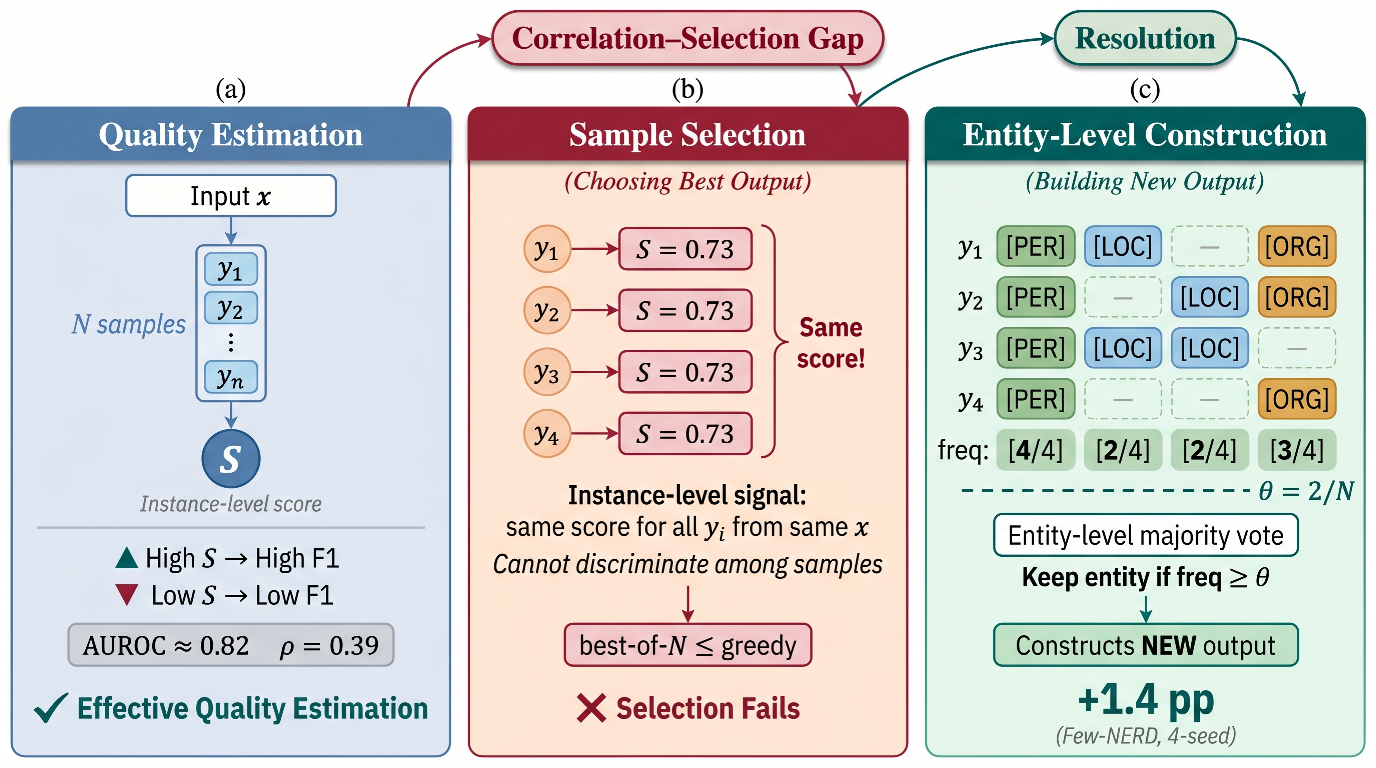
\includegraphics[width=\textwidth]{fig_overview}
\caption{Overview of the correlation-selection gap (diagnostic sequence, not causal chain). Representative values across datasets: AUROC from CoNLL EM; Spearman $\rho$ and entity-construction gain from Few-NERD (Qwen3-8B, $N{=}8$, $T{=}1.0$; Tables~\ref{tab:multiseed},~\ref{tab:entity_construction}). \textbf{Left}: consistency signals estimate instance quality. \textbf{Center}: instance-level signals assign identical scores to all $N$ candidates, so selection cannot outperform greedy. \textbf{Right}: LP-weighted entity construction ($\theta{=}2/N$) yields conditional gains ($+1.40$\,pp on Few-NERD; \S\ref{sec:prescriptive}).}
\label{fig:overview}
\end{figure*}

Our investigation proceeds in three stages:
\begin{enumerate}[nosep]
\item \textbf{Discover} [\S\ref{sec:qe_results}].
QE signals achieve strong instance-level discrimination (AUROC up to $0.82$); while \citet{yao2026consistency} report task-level correlation, our instance-level decomposition reveals why this does not translate into selection gains.
\item \textbf{Diagnose} [\S\ref{sec:selection_gap}, \S\ref{sec:adaptive}, \S\ref{sec:theory}].
A diagnostic cascade quantifies failure mechanisms at entity level; \citet{yun2025price} describe diversity collapse qualitatively, we provide quantitative decomposition through degeneracy ($D$), alignment ($\alpha$), and LP range. A necessary condition bound confirms $\alpha$ as the binding constraint (3--12\% recovery ratio). Hidden-state probes expose an introspection boundary (probe AUROC up to $0.88$ vs.\ ESJ ${\approx}0.50$; Appendix~\ref{sec:mechanistic}).
\item \textbf{Construct (conditional)} [\S\ref{sec:prescriptive}].
Entity-level construction yields $+1.40$\,pp on Few-NERD where the cascade identifies favorable conditions (low degeneracy, positive LP--F1 alignment), but inverse scaling elsewhere; this validates the framework's prescriptive scope.
\end{enumerate}

The paper is organized as follows: \S\ref{sec:related} contextualizes our contributions; \S\ref{sec:method} defines the diagnostic framework; \S\ref{sec:selection_gap} establishes the correlation-selection gap; \S\ref{sec:adaptive} evaluates adaptive methods; \S\ref{sec:theory_scaling} provides scaling analysis; \S\ref{sec:experiments} presents cross-dataset results.
